\documentclass{beamer}
\usetheme{dianahep}

%
% Title definitions
%

\title{Community White Paper: \\
       A Roadmap for HEP Software and Computing \\
       Status and Plans}
\author{Peter Elmer - Princeton University \\
\date{10 November, 2016 \\ CMS Offline and Computing Week}

\begin{document}
\maketitle
%\insertframenumber/\inserttotalframenumber

%
% Presentation body
%

\setbeamertemplate{footline}[frame number]

%\begin{frame}
\frametitle{Introduction}

\begin{itemize}
\item You only get out what you put in...
\end{itemize}

\end{frame}




\begin{frame}
\frametitle{A Software ``Upgrade'' for HL-LHC and 2020s HEP?}

Looking forward to the next 10 years, we see a number of challenges for HEP software and computing:

\begin{itemize}
\item {\bf Scale:} The HL-LHC will integrate 100 times the current data, with significantly increased data (pileup) and detector complexity.
\item {\bf Performance/cost:} Estimates of computing needs run faster than Moore's Law by factors of 3-30
\item {\bf Technology/Market evolution:} the return of heterogeneity; technology change will also make it challenging to exploit Moore's Law without software evolution.
\item {\bf Sustainability:} Most of the current software, which defines our capabilities, was designed 15-20 years ago: there are many software sustainability challenges.
\end{itemize}

\end{frame}




\begin{frame}
\frametitle{Why Software? Software is {\em the} Cyberinfrastructure}

\begin{figure}[htbp]
\begin{center}
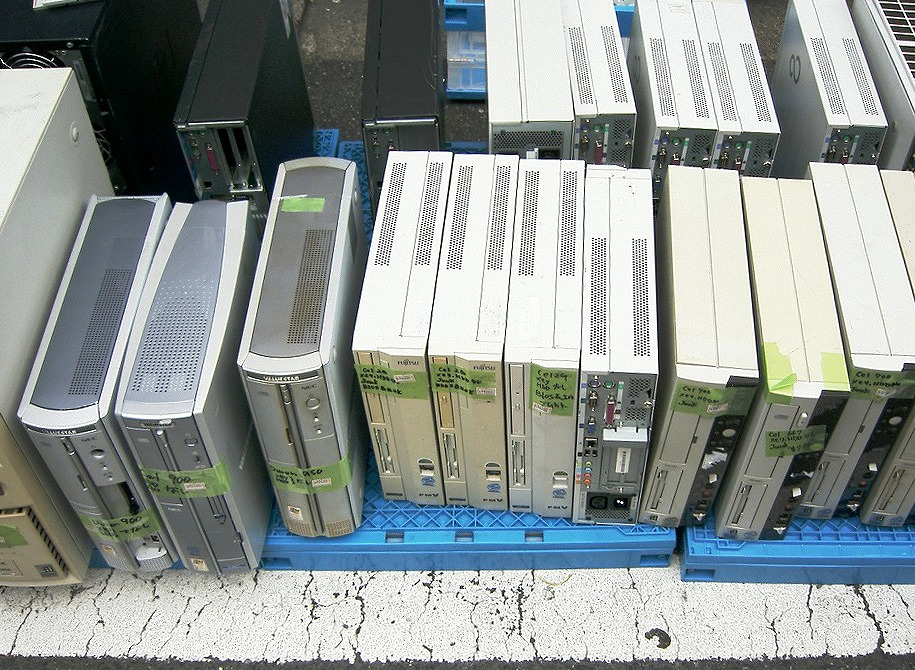
\includegraphics[width=0.7\textwidth]{images/Junk_desktop_personal_computer.jpg}
%\caption{}
%\label{fig:example2}
\end{center}
\end{figure}

\begin{center}
\small{Computer hardware is a consumable. \\ Software is what we keep, and invest in, over time.}
\end{center}

\end{frame}




\begin{frame}
\frametitle{Estimates of Resource Needs for HL-LHC (WLCG)}

\begin{figure}[htbp]
\begin{center}
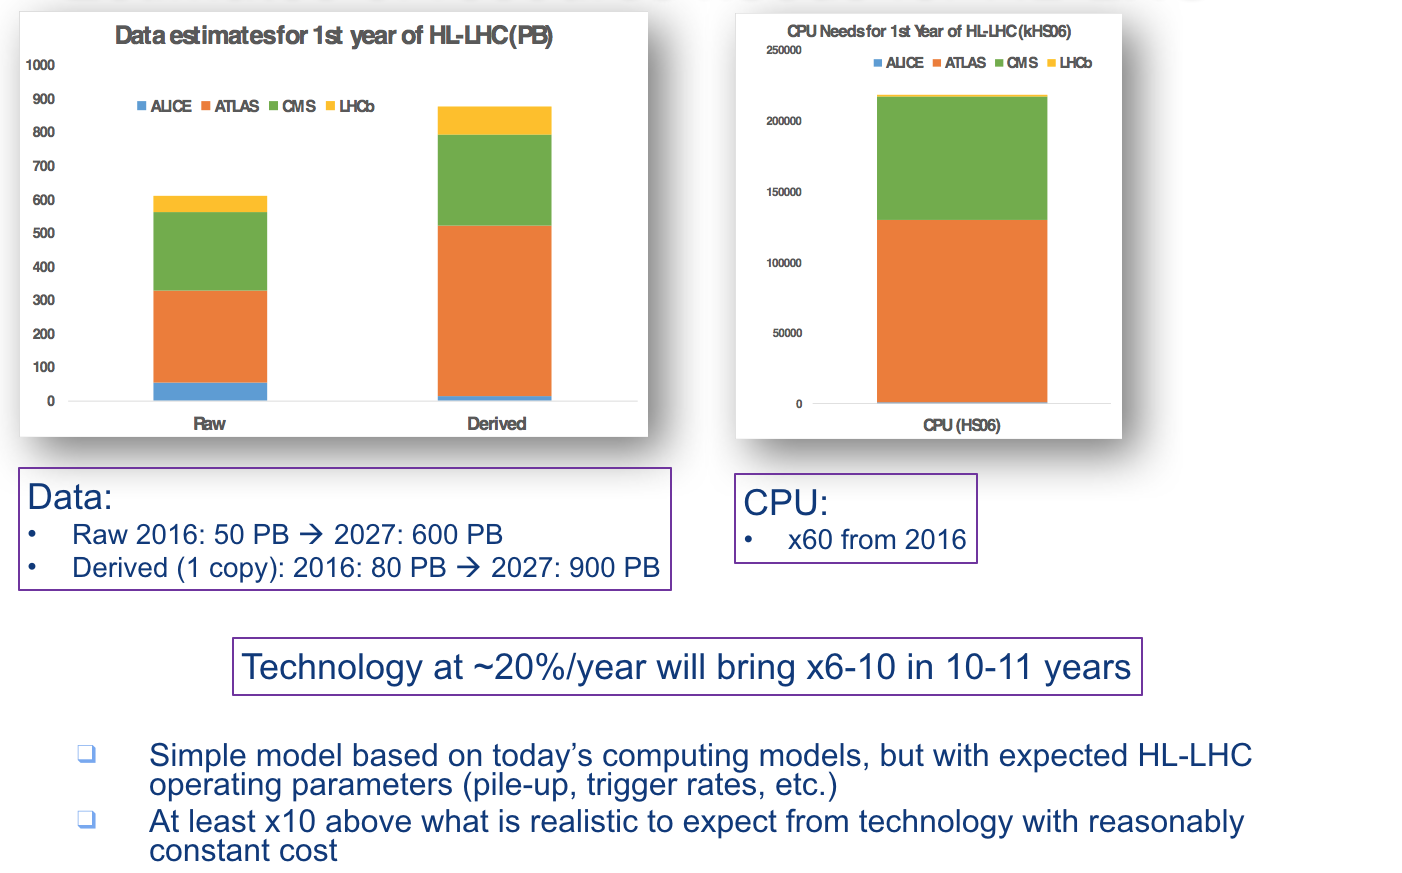
\includegraphics[width=0.9\textwidth]{images/20161008-wlcg-intro-ian-bird-slide-10.png}
\end{center}
\end{figure}

\begin{center}
\small{(Slide from WLCG Workshop Intro, Ian Bird, 8 Oct, 2016)}
\end{center}

\end{frame}




%\begin{frame}
\frametitle{Processor evolution - Power dissipation vs Time}

\begin{columns}[T] % align columns

\begin{column}{.48\textwidth}
\begin{figure}[htbp]
\begin{center}
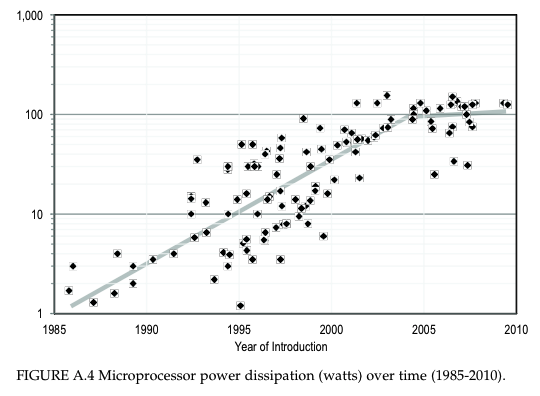
\includegraphics[width=1.0\textwidth]{images/moore1.png}
\end{center}
\end{figure}
\end{column}%

\hfill%

\begin{column}{.48\textwidth}
\small{Power density limitations in processors fundamentally changed the game from about 2005.}
\end{column}%

\end{columns}


\end{frame}



\begin{frame}
\frametitle{Processor evolution and software impact}

\begin{columns}[T] % align columns

\begin{column}{.48\textwidth}
\begin{figure}[htbp]
\begin{center}
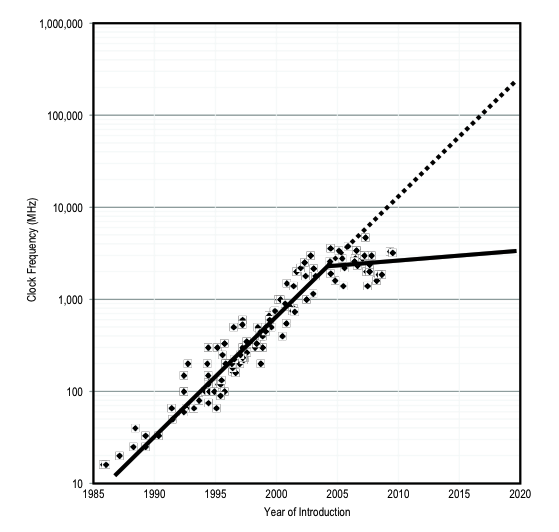
\includegraphics[width=1.0\textwidth]{images/moore2.png}
\end{center}
\end{figure}
\begin{center}
\small{Clock Frequency vs Time}
\end{center}
\end{column}%

\hfill%

\begin{column}{.48\textwidth}
\begin{itemize}
\item Single core performance has stalled, leading to multi/manycore and specialization
\item To even realize Moore's Law gains, we are pushed towards parallelization of algorithms and design for performance.
\item The software designs and implementations themselves need to evolve, not just be recompiled
\end{itemize}
\end{column}%

\end{columns}

\end{frame}



\begin{frame}
\frametitle{Back to heterogeneous systems?}

Building the worldwide distributed LHC computing grid was largely made possible by the convergence on Linux on (commodity) Intel x86 processors around the year 2000. Building the WLCG at this scale in the heterogeneous workstation era would have been quite difficult. For better or for worse, heterogeneity is returning:

\begin{itemize}
\item Diversity of computing processor architectures (general purpose cores vs specialized processors)
\item Owned vs commercial/cloud providers
\item Some pressure to use systems traditionally designed for other types of applications (e.g.\ HPC/supercomputer as opposed to HTC/high-throughput systems)
\item Possible further commoditizing market pressures (e.g. mobile)
\end{itemize}

\end{frame}



\begin{frame}
\frametitle{What is software sustainability?} 
\begin{itemize}
\item {\bf Dependent Infrastructure:} Will the infrastructure element continue to provide the same functionality in the future, even when the other parts of the infrastructure on which the element relies change?
\item {\bf Collaborative Infrastructure} Can the element be combined with other elements to meet user needs, as both the collaborative elements and the individual elements change?
\item {\bf New Users:} Is the functionality and usability of the infrastructure element clearly explained to new users? Do users have a mechanism to ask questions and to learn about the element?
\item {\bf Existing Users:} Does the infrastructure element provide the functionality that current users want? Is it modular and adaptable so that it can meet the future needs of the users?
\item {\bf Science:} Does it incorporate and implement new science and theory as they develop?
\end{itemize}

\tiny{ Katz, D.S. \& Proctor, D., (2014). A Framework for Discussing e-Research Infrastructure Sustainability. Journal of Open Research Software. 2(1), p.e13. DOI: http://doi.org/10.5334/jors.av}
\end{frame}





\begin{frame}
\frametitle{HEP Software Foundation (HSF)}

\begin{columns}[T] % align columns

\begin{column}{.75\textwidth}
The HSF (http://hepsoftwarefoundation.org) was created 1.5 years ago as a means for organizing our community to address the software challenges of future projects such as the HL-HLC. The HSF has the following objectives: 
\end{column}%

\hfill%

\begin{column}{.20\textwidth}
\begin{figure}[htbp]
\begin{center}

\includegraphics[width=1.0\textwidth]{images/hsf_logo_angled.png}
\end{center}
\end{figure}
\end{column}%

\end{columns}

\vskip 0.1in

\begin{itemize}
\item Catalyze new common projects
\item Promote commonality and collaboration in new developments to make the most of limited resources
\item Provide a framework for attracting effort and support to S\&C common projects (new resources!)
\item Provide a structure to set priorities and goals for the work
\end{itemize}

%An initial set of collaborative activities have begun (see recent HSF workshop 
%at LAL-Orsay). 


\end{frame}




%\begin{frame}
\frametitle{Collaboration Challenges}

\begin{itemize}
\item The LHC and other HEP experiments cannot afford to undertake this software revolution independently
  \begin{itemize}
  \item There are many common software packages that would require common efforts, thus coordination
  \item General wish to increase the level of commonality and re-use
  \end{itemize}
\item Require the collaboration of the whole HEP community to ensure evolution and sustainability
  \begin{itemize}
  \item Show a common and coherent roadmap to funding agencies
  \item Establish structures to facilitate contributions to the HEP software stack 
  \end{itemize}
\item The adoption of a collective response will help to meet the challenges using available expertise and resources and within the required timeline
\end{itemize}

\end{frame}



\begin{frame}
\frametitle{HEP Software Ecosystem}

\begin{figure}[htbp]
\begin{center}
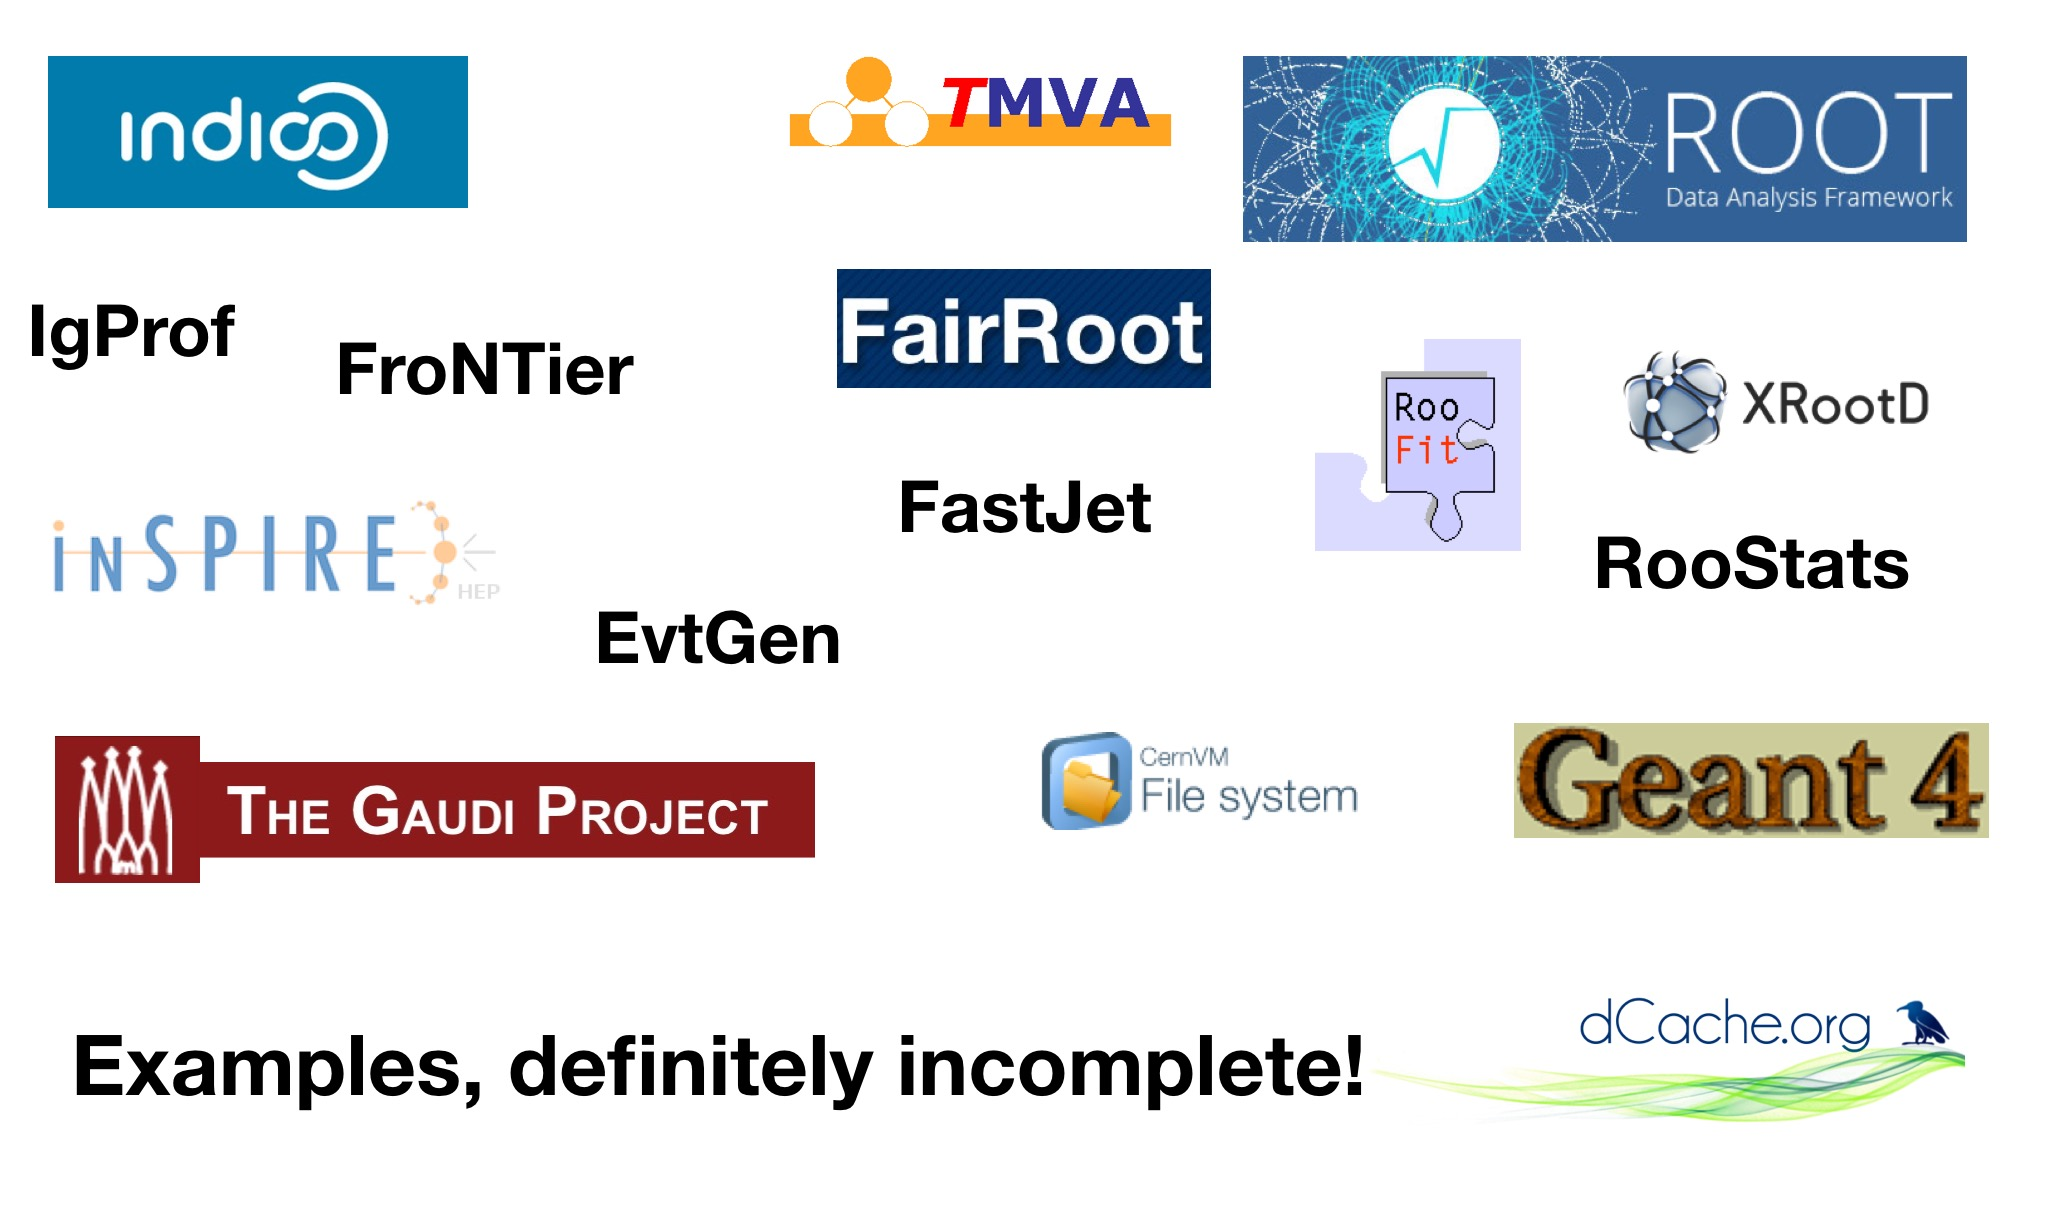
\includegraphics[width=0.9\textwidth]{images/hep-software-ecosystem.jpg}
\end{center}
\end{figure}

\end{frame}



\begin{frame}
\frametitle{Recent/Nascent Cross-experiment Collaborations}

\begin{itemize}
\item Experiment frameworks
  \begin{itemize}
  \item Gaudi, FAIRRoot, CMSSW/Art
  \end{itemize}
\item Common Conditions Data Project
  \begin{itemize}
  \item Discussion/cooperation between ATLAS, Belle II, CMS and LHCb
  \end{itemize}
\item Common Software Build and Packaging Tools efforts
  \begin{itemize}
  \item Working group of HSF comparing HEP and non-HEP solutions
  \end{itemize}
\item Cooperation on Reconstruction Software
  \begin{itemize}
  \item ``Connecting the Dots'' tracking workshop, HSF sessions 
  \end{itemize}
\item AIDA2020 (EU funded)
  \begin{itemize}
  \item DD4hep for detector description, PODIO data model library (LCD, FCC, potentially LHCb)
  \end{itemize}
\item DIANA (Data Intensive ANAlysis) (NSF Funded)
  \begin{itemize}
  \item 4-year project on analysis software, including ROOT and its ecosystem
  \end{itemize}
\end{itemize}

\end{frame}




%\begin{frame}
\frametitle{HSF - Initial Activities}
\begin{itemize}
\item 
\item 
\end{itemize}

\end{frame}



%\begin{frame}
\frametitle{Coping with HL-LHC Needs}

\begin{itemize}
\item To cope with the enormous expected computing demands for the HL-LHC, we have two solutions:
  \begin{itemize}
  \item Invest in more computing: more hardware, more centers, ...
  \item Invest in better software
  \item or a combination of both
  \end{itemize}
\item What is ``better'' software?
  \begin{itemize}
  \item Better algorithms, new ideas
  \item Better adapted to the current and future hardware architectures
  \item Better optimisations
  \item Better quality
  \item Better sustainability
  \end{itemize}
\end{itemize}

\end{frame}




\begin{frame}
\frametitle{Defining Longer-term Strategy}

\begin{itemize}
\item HL-LHC computing requires a major `software upgrade'
\item A Community White Paper (CWP) on the overall strategy and roadmap 
for software and computing has been proposed
  \begin{itemize}
  \item Initiated as WLCG charge to the LHC experiments and HSF as a step towards the LHC experiment TDRs in advance of HL-LHC
  \item The scope should not be restricted only to HL-LHC
  \item Some early software components could be built, tested and used by experiments in LHC Run3
  \end{itemize}
\item Organised by the HEP Software Foundation (HSF)
\item Paper to be delivered by Summer 2017
\item It should play a role in discussing possible funding scenaries for a ``software upgrade''.
\end{itemize}


\end{frame}



\begin{frame}
\frametitle{Community White Paper (CWP)}

\begin{itemize}
\item The CWP should identify and prioritise the software research and development investments required:
   \begin{itemize} 
   \item to achieve improvements in software efficiency, scalability and performance and to make use of the advances in CPU, storage and network technologies
   \item to enable new approaches to computing and software that could radically extend the physics reach of the detectors
   \item to ensure the long term sustainability of the software through the lifetime of the HL-LHC
   \end{itemize} 
\vskip 0.15in
\item We need to engage the HEP community in this process through a series of workshops
   \begin{itemize} 
   \item Initiated as an HL-LHC planning process
   \item Aiming for a broader participation (LHC, neutrino program, Belle II, linear collider so far)
   \end{itemize} 
\end{itemize}

\end{frame}



\begin{frame}
\frametitle{Likely constraints to fund a ``Software Upgrade''}

It appears unlikely that significant increases in investments in software 
will be made by funding agencies purely from particle physics budgets 
and/or into individual experiments. Other opportunities do perhaps exist,
but often imply constraints, for example:

\begin{itemize}
\item Investments into software impacting multiple experiments 
\item Investments into development with impact beyond particle physics 
\item Investments into development permitting use of computing facilities (e.g. HPC) planned for other non-HEP purposes
\item Investments requiring collaborations with Computer Science or Industry
\end{itemize}

Building the LHC software in use today was possible without too many such constraints. The good news is that the community (with an existing LHC computing system) is better positioned today to make effective progress even with such constraints.

\end{frame}



%\begin{frame}
\frametitle{Derived Plans and Proposals} 
The CWP should be the document from which specific plans/proposals can be derived. The US NSF, for example, has indicated a possible path forward to real resources (next slide) to fund a part of such an upgrade project. In parallel to the CWP process proposed here we will prepare a ``Strategic Plan'' for the NSF.
\vskip 0.15in
It should also provide a better context for engaging computer scientists, other sciences and industry (e.g. through CERN Openlab)
\vskip 0.15in
As a community we should be pursuing and preparing the ground for these opportunities in parallel to the preparation of the CWP.
\end{frame}




\begin{frame}
\frametitle{Status}

\noindent 
The proposal for a general Community Roadmap has been widely discussed with all of the LHC experiments and the HEP Software Foundation (HSF). There is broad support for the idea. \\
\vskip 0.1in
The CWP roadmap plan, to be carried out by HSF, was presented to the LHCC. It fits with the current notion of HL-LHC computing TDRs in $\sim$2019-2020.\\
\vskip 0.1in
WLCG has produced a charge for this CWP to the HSF and the LHC experiments (see separate link) with an aim to complete it by the end of August, 2017. \\
\vskip 0.1in
The HSF has begun the process of organizing working groups, engaging HEP beyond the LHC experiments and planning for dedicated workshops. Sessions at existing meetings can also be used when possible. \\

\end{frame}




\begin{frame}
\frametitle{Community Roadmap Process}

We propose a series of workshops over the next year to build the community roadmap:

\begin{itemize}
\item Initial presentation and organization this month (at WLCG workshop and CHEP, etc.)
  \begin{itemize}
  \item Flesh out the charges and attract interested individuals to the WGs
  \end{itemize}
\item A ``kick-off'' workshop at UC San Diego on 23-26 Jan 2017
  \begin{itemize}
  \item Start real work after a few months post-CHEP gestation in the WGs
  \item Discussions on more controversial topics, find path to consensus
  \item Develop plans and responsibilities for delivering white paper by summer 2017
  \end{itemize}
\item Possible ``topical'' workshops between Jan-Jun 2017, building on existing community activities when possible (e.g.\ DPHEP, Reco Algorithms Forum/CTD, IML)
\item A final workshop in summer 2017 (in Europe, near CERN?)
\end{itemize}

\end{frame}



\begin{frame}
 \frametitle{What should the community roadmap process accomplish?}
Going back to the subset of HSF goals I listed earlier:

\begin{itemize}
\item Catalyze new common projects
\item Promote commonality and collaboration in new developments to make the most of limited resources
\item Provide a framework for attracting effort and support to S\&C common projects (new resources!)
\item Provide a structure to set priorities and goals for the work
\end{itemize}

The workshop process, the community roadmap white paper and (simultaneously) the pursuit of specific plans/proposals will support precisely these goals.

\end{frame}




%\begin{frame}
\frametitle{Software and Computing for the HL-LHC Era }

We don't have precise totals for the cost of global LHC computing 
effort due to the ``in kind'' nature of most of the contributions and different accounting systems.
As a data point we do know that the U.S.\ DOE and NSF jointly invest 
$ \approx \$ 35 $M/year in
ATLAS and CMS software and computing projects, about half in hardware plus operations,
about half in software professionals.
Extrapolating we can conclude that the LHC funding agencies, worldwide, 
likely invest of order $ \$ 100-150 $M/year in these enterprises.

The event rate anticipated for the HL-LHC era is 100 times greater than Run1,
and even assuming the experiments significantly reduce the
amount of data stored per event,
they will be constrained primarily by costs and funding levels,
not by scientific interest.
One long-term goal of a software upgrade for HL-LHC
will be maximizing the return-on-investment to enable break-through
scientific discoveries using the  HL-LHC detectors.


\end{frame}



\begin{frame}
\frametitle{Possible routes to a ``Software Upgrade''}

\begin{itemize}
\item If we are aiming at a larger ``software upgrade'' project towards the HL-LHC, an additional ingredient is to find (or liberate/reallocate) the resources to realize this roadmap. 
\item We need both initial exploratory R\&D and eventual development projects!
\item In the US, both the NSF and the DOE have at least the notion of eventual resources and/or organization for new common projects in HEP (NSF: SI2, DOE: HEP CCE)
  \begin{itemize}
   \item The US NSF has funded a ``conceptualization'' (planning) project with a possible path towards a ``Software Institute''.
   \item The US DOE has seeded the ``Center for Computing Excellence'' with some initial resources. 
  \end{itemize}
\item We hope that a clear community roadmap will bring these and other partners together for an HL-LHC software upgrade.
\end{itemize}

\end{frame}




\begin{frame}
\frametitle{Practicalities: HSF Google Groups}

The following Google Groups are relevant:

\begin{itemize} 

\item Group for discussion of Community White Paper
  \begin{itemize} 
  \item {\color{blue} \url{https://groups.google.com/forum/\#!forum/hsf-community-white-paper}}
  \end{itemize} 

\item General announcement group for community messages (low traffic)
  \begin{itemize} 
  \item {\color{blue} \url{https://groups.google.com/forum/\#!forum/hep-sw-comp}}
  \end{itemize} 

\item Community Discussion list
  \begin{itemize} 
  \item {\color{blue} \url{https://groups.google.com/forum/\#!forum/hep-sf-forum}}
  \end{itemize} 

\item Specific group for US NSF Software Institute Conceptualization
  \begin{itemize} 
  \item {\color{blue} \url{https://groups.google.com/forum/\#!forum/s2i2-hep}}
  \end{itemize} 

\end{itemize} 

\end{frame}



\begin{frame}
\frametitle{Practicalities: Charges for CWP Working Groups}


\begin{itemize} 
\item Over the next weeks we will be formulating charges for the CWP working groups.
\item Templates for drafting these charges are in google docs.
\item The overall WLCG HSF charge and links to individual WG charge google docs (in preparation) can be found at:
   \begin{itemize}
   \item {\color{blue} \url{http://bit.ly/2dcZZqa}}
   \end{itemize}
\item To view and/edit these charges you will need to be subscribed to:
   \begin{itemize}
   \item {\color{blue} \url{https://groups.google.com/forum/\#!forum/hsf-community-white-paper}}
   \end{itemize}
\item These google docs are just to draft the charges and allow people to self-organize and start discussions. Eventual proper documents (e.g. in latex) can switch elsewhere (e.g. github).
\end{itemize} 

\end{frame}



%\begin{frame}
\frametitle{Detector Simulation, Triggering, Event Reconstruction and Visualization} 
\scriptsize{
Challenges surrounding high pile-up simulation,
including the CPU resources needed for large statistics samples
needed to compare with data from high trigger rates, high memory
utilization, generation and handling of the large (min-bias) samples
needed to achieve accurate description of high pile-up collision
events, and a flexible simulation strategy capable of a broad
spectrum of precision in the detector response, from ``fast''
(e.g. parametric) simulation optimized for speed to full simulation
in support of precision measurements and new physics searches
(e.g. in subtle effects on event kinematics due to the presence of
virtual particles at high scale).
Software required to emulate upgraded detectors (including the
trigger system) and support determination of their optimal
configuration and calibration.
Software in support of triggering
during the HL-LHC, including algorithms for the High-level Trigger,
online tracking using GPUs and/or FPGAs, trigger steering, event
building, data ``parking'' (for offline trigger decision), and data
flow control systems. New approaches to event reconstruction, in
which the processing time depends sensitively on instantaneous
luminosity, including advanced algorithms, vectorization, and
execution concurrency and frameworks that exploit many-core
architectures. In particular, charged particle tracking is expected
to dominate the event processing time under high pile-up
conditions. Visualization tools, not only in support of upgrade
detector configurations and event displays, but also as a research
tool for data analysis, education, and outreach using modern tools
and technologies for 3D rendering, data and geometry description and
cloud environments.
}
\end{frame}



%\begin{frame}
\frametitle{Data Access and Management, Workflow and
Resource Management}
\scriptsize{ 
Data handling systems that scale to the Exabyte level during the
HL-LHC era and satisfy the needs of physicists in terms of metadata
and data access, distribution, and replication. Increasing
availability of very high speed networks removes the need for CPU
and data co-location and allows for more extensive use of data
access over the wide-area network (WAN), providing failover
capabilities, global data namespaces, and caching. Event-based data
streaming as complementary to the more traditional dataset-based or
file-based data access, which is particularly important for
utilizing opportunistic cycles on HPCs, cloud resources, and campus
clusters where job eviction is frequent and stochastic. Workflow
management systems capable of handling millions of jobs running on a
large number of heterogeneous, distributed computing resources, with
capabilities including whole-node scheduling, checkpointing, job
rebrokering, and volunteer computing. Systems for measurement and
monitoring of the networking bandwidth and latency between resource
targets and the use of this information in job
brokering. Software-defined networking technologies which enable
networks to be configurable and schedulable resources for use in the
movement of data.
}

\end{frame}



%\begin{frame}
\frametitle{ Physics generators, Data Analysis and Interpretation, Data and Software Preservation}
\scriptsize{ 
There are many theory challenges in the HL-LHC era, among them are
improving the precision of SM calculations, better estimation of
systematic uncertainties, and elucidation of promising new physics
signals for the experiments. Software needed to make connection
between observations and theory include matrix element generators,
calculation of higher-order QCD corrections, electroweak
corrections, parton shower modeling, parton matching schemes, and
soft gluon resummation methods. Physics generators that employ
concurrency and exploit many-core architectures will play an
important role in HL-LHC, as well better sharing of code and
processing between LHC experimenters and phenomenologists. Data
analysis frameworks that include parallelization, optimized event
I/O, data caching, and WAN-based data access. Analysis software
that employs advanced algorithms and efficiently utilizes many-core
architectures. Tools and technologies for preservation and reuse of
data and software, preservation and re-interpretation of physics
results, analysis providence and workflow ontologies, analysis
capture, and application packaging for platform abstraction. Future
software repositories and build platforms that leverage advances in
these areas and improved software modularity and quality control
that will allow a broader community of people to effectively
contribute to software in the HL-LHC era.}

\end{frame}



\begin{frame}
\frametitle{Practicalities: Possible Working Groups}
\begin{table}[h!]
\tiny
\centering
\label{tab:table1}
\begin{tabular}{|l|l|}
\hline
Detector Simulation & full and fast simulations, hi-pileup environments \\ \hline

Triggering & algorithms, GPUs and/or FPGAs \\ \hline

Event Reconstruction & new approaches to event reconstruction \\ \hline

Visualization & tools for data analysis, education, and outreach \\ \hline

Data Access and Management & scaling to the exabyte level \\ \hline

Workflow and Resource Management & millions of jobs in heterogenous systems \\ \hline

Physics generators & better models, better precision, code optimisations \\ \hline

Data Analysis and Interpretation & efficient use of many-core, modern techniques \\ \hline

Data and Software Preservation & preservation and reuse of data and software \\ \hline

Software Development, Deployment & \\
and Validation/Verification & improved modularity and quality, contribution \\ \hline

Computing Models, Facilities, & \\
Distributed Computing & \\ 
Various Aspects of Technical Evolution & \\ 
(Software Tools, Hardware) & range of possible models, costing, technology \\ \hline

Security and Access Control & \\ \hline

Careers, Staffing and Training & perhaps in a separate concurrent white paper \\ \hline

Machine Learning & \\ \hline

Conditions Database & \\ \hline

Event Processing Frameworks & \\ \hline
\end{tabular}
\end{table}

\begin{center}
\small{More details in links at \color{blue} {\url{http://bit.ly/2dcZZqa}}}
\end{center}

\end{frame}



\begin{frame}
\frametitle{Practicalities: Documents}

\begin{itemize}
\item The end goal here is a single CWP roadmap for the community. 
\item The first step is building working groups and defining specific charges
\item The process of putting together the CWP should generate a series of narrower topical documents from the working groups. (Much like the Snowmass process, for example.)
\item Existing public documents are something we will build upon, e.g. the Snowmass Computing documents, the DOE HEP-CCE documents, the WLCG Run2 Computing Model Update, the CERN Openlab whitepaper, etc.
\item The specific mechanics of assembling the CWP document itself will be defined at the Jan2017 SDSC HSF CWP workshop
\end{itemize}

\end{frame}




\begin{frame}
\frametitle{Discussion questions}

\begin{itemize}
\item How can we best organize to produce a consensus roadmap for the Community White Paper? What is missing from the proposed process?
\item How can we best address the three CWP goals?
   \begin{itemize}
   \item to achieve improvements in software efficiency, scalability and performance and to make use of the advances in CPU, storage and network technologies
   \item to enable new approaches to computing and software that could radically extend the physics reach of the detectors
   \item to ensure the long term sustainability of the software through the lifetime of the HL-LHC
   \end{itemize}
\item In practice how do we re-examine the organizational processes by which the HEP community and the experiments collaborate?
\item What opportunities do we have for funding a ``software upgrade'' to address these challenges?
\end{itemize}



\end{frame}



\begin{frame}
\frametitle{HEP Software Ecosystem}

\begin{figure}[htbp]
\begin{center}
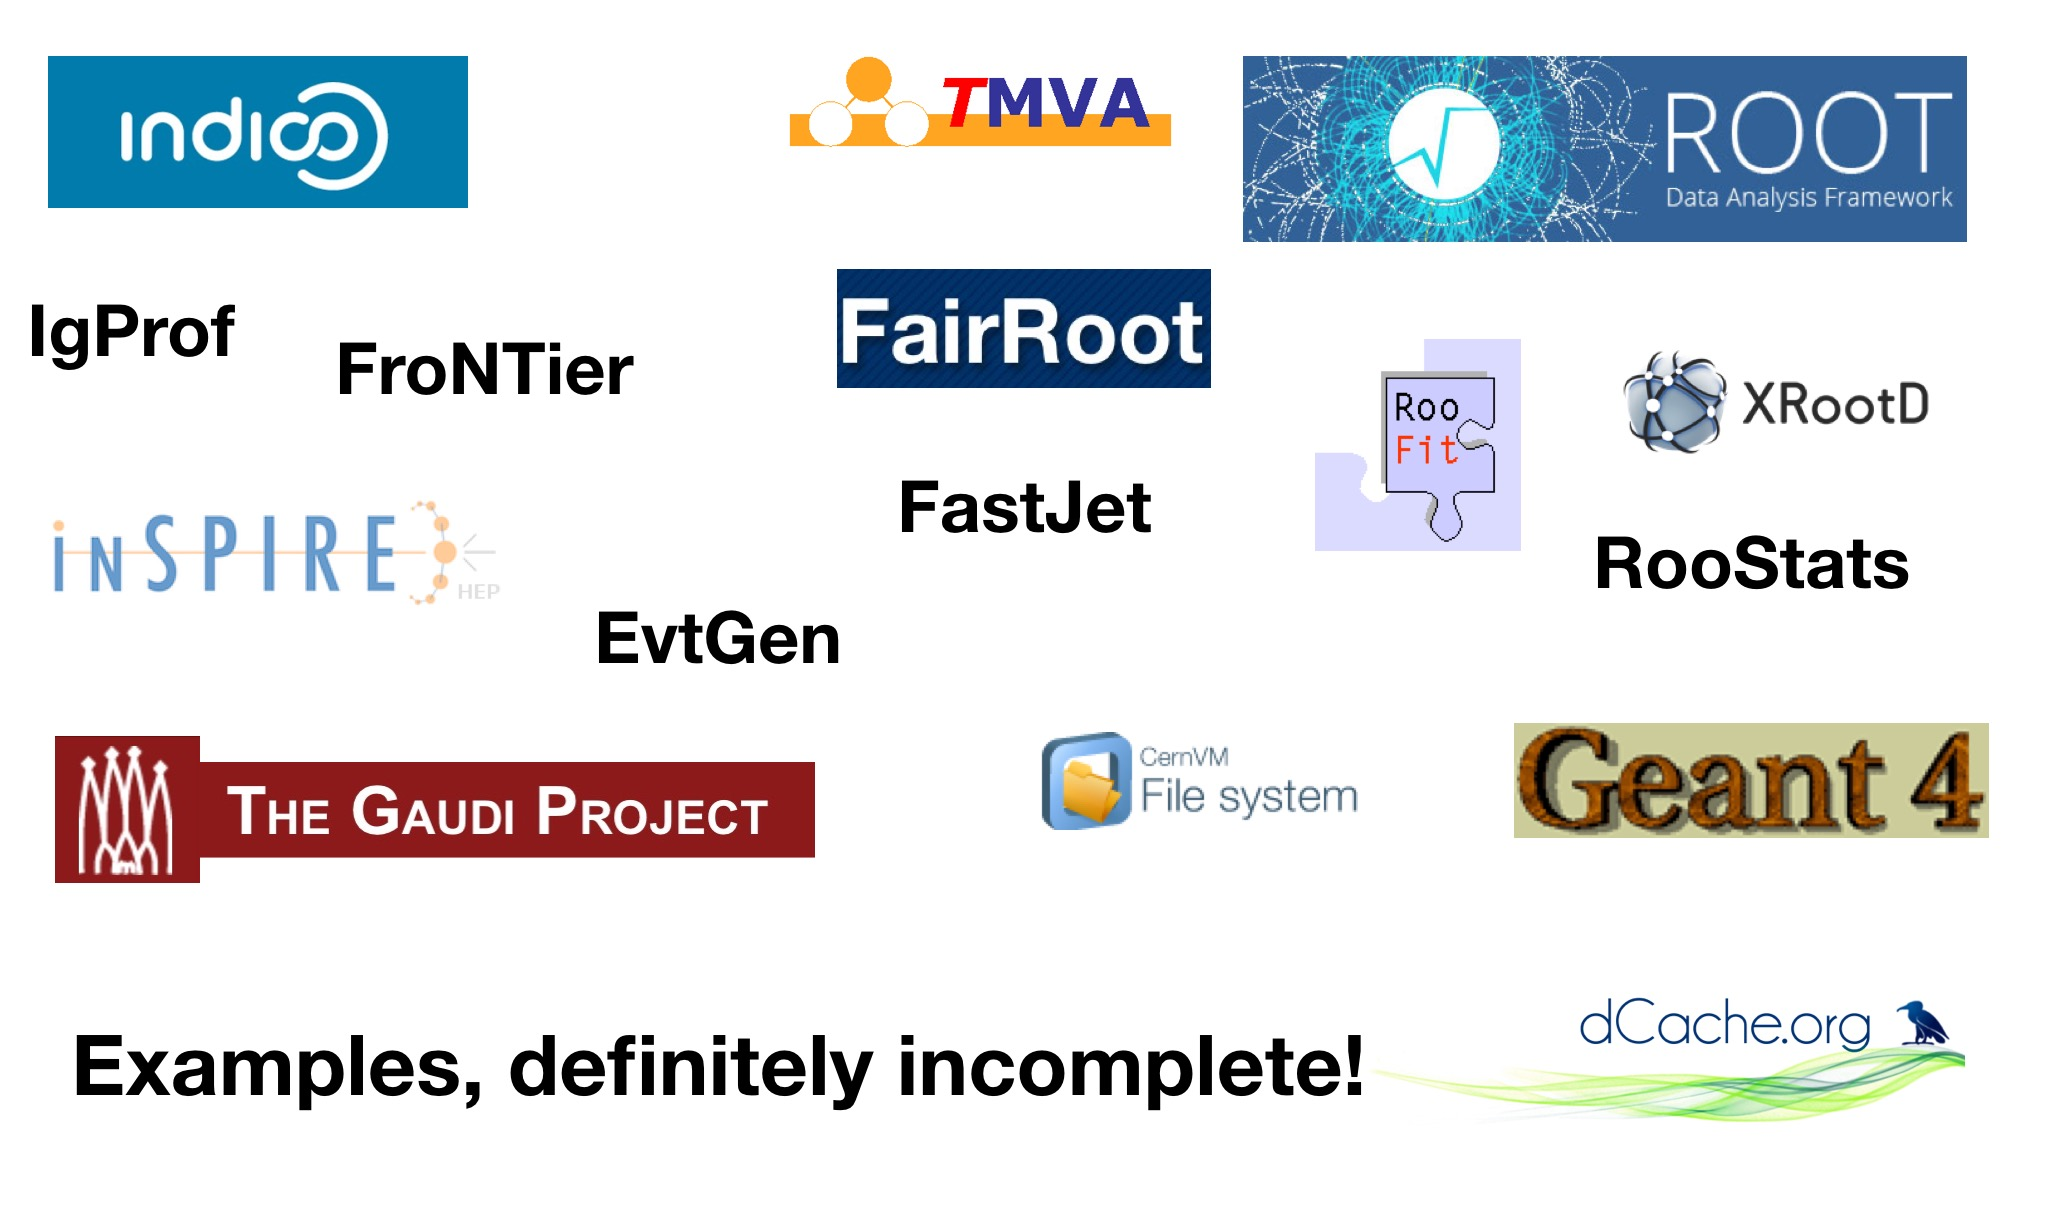
\includegraphics[width=0.9\textwidth]{images/hep-software-ecosystem.jpg}
\end{center}
\end{figure}

\end{frame}




\end{document}


